%---------------------------- Beginning of preamble


%-------- document class
% comment this line if you want to print the presentation and uncomment the next one
\documentclass[8pt, hide notes]{beamer} 
% comment this line if you want to show the presentation and uncomment the previous one
%\documentclass[8pt, handout]{beamer} 


%-------- general layout
\mode<presentation>
{
  
  
  
  	%---- themes
  	\usetheme{Antibes}
  	%\usetheme{Singapore}
  	%\usetheme{Warsaw}


	%color theme
	\usecolortheme{lily}

	  %for math characters
  	\usefonttheme[onlylarge]{structuresmallcapsserif}

	%remove navigation symbols
	\setbeamertemplate{navigation symbols}{}

	%left margin 
	\setbeamersize{text margin left=0.5cm}

	%dark blue for normal text
	\definecolor{MyDarkBlue}{rgb}{0.0235,0.1569,0.4745}
	\setbeamercolor{normal text}{fg = MyDarkBlue}
	\definecolor{Mygrey}{RGB}{181,181,181}

	
	%white for background text color
	\setbeamercolor{structure}{bg = white}
		
	%---- headline
	% black and white for headline and footline
	\setbeamercolor{section in head/foot}{bg = white, fg=black}
	\setbeamercolor{subsection in head/foot}{bg = white, fg=black}
	\setbeamercolor{title in head/foot}{bg = white, fg=black}	
	
	%What do you want in your header? by default, there is the current subsection
	
	%if you want to insert a complete navigation	
	\setbeamertemplate{headline}
	{\vskip5pt
	}%--


	%---- frame title
	\setbeamertemplate{frametitle}
	{%--
	\textcolor{MyDarkBlue}{\insertframetitle}
		\hfill 
	\rule{\textwidth}{0.5pt}
	}%--
	
	
	%---- footline	
	%add frame number and logo
	\setbeamertemplate{footline}
	{%--
	   %you can adjust the left and right white space with leftskip and rightskip
	\begin{beamercolorbox}[ht=2.5ex,dp=1.125ex,
	    leftskip=.15cm,rightskip=.15cm plus1fil]{title in head/foot}
	     useR 2019 conference -- C. Dutang -- \insertshortdate	
	     \hfill
	     \insertframenumber/\inserttotalframenumber
	\end{beamercolorbox}
  	}%--
}

%-------- macro latex



%theorems
\newtheorem{mydef}{Definition}
\newtheorem{mytheo}{Theorem}
\newtheorem{mycor}{Corollary}
\newtheorem{myprop}{Proposition}
\newtheorem{mylemma}{Lemma}

\usepackage{bm}

%sets
\newcommand{\N}{\ensuremath{\mathbb{N}}}
\newcommand{\C}{\ensuremath{\mathbb{C}}}
\newcommand{\R}{\ensuremath{\mathbb{R}}}
\newcommand{\X}{\ensuremath{\mathbb{X}}}
\newcommand{\Y}{\ensuremath{\mathbb{Y}}}

\newcommand{\calN}{\mathcal N}
\newcommand{\calF}{\mathcal F}
\newcommand{\calE}{\mathcal E}
\newcommand{\calL}{\mathcal L}
\newcommand{\calC}{\mathcal C}
\newcommand{\calT}{\mathcal T}
\newcommand{\calX}{\mathcal X}
\newcommand{\calD}{\mathcal D}

\newcommand{\bx}{\boldsymbol{x}}
\newcommand{\by}{\boldsymbol{y}}
\newcommand{\bz}{\boldsymbol{z}}
\newcommand{\bX}{\boldsymbol{X}}
\newcommand{\bY}{\boldsymbol{Y}}
\newcommand{\bZ}{\boldsymbol{Z}}


%text style
\newcommand{\pkg}{\textbf}
\newcommand{\sigle}{\textsc}
\newcommand{\code}{\texttt}
\newcommand{\soft}{\textsf}
\newcommand{\tinym}[1]{\mbox{\tiny $#1$}}
\newcommand{\bleu}[1]{{\color{MyDarkBlue}#1}}
\newcommand{\red}[1]{{\color{MyDarkBlue}#1}}

\newcommand{\dix}[1]{{\footnotesize x10\textsuperscript{-#1}}}




%math
\DeclareMathOperator{\id}{id}
\DeclareMathOperator{\diag}{diag}
\DeclareMathOperator{\rank}{rank}
\DeclareMathOperator{\atan}{atan}

\newcommand{\abs}[1]{\left\lvert#1\right\rvert}
\newcommand{\bigo}[1]{\mathcal O \hskip -0,2em \left(#1\right)}
\newcommand{\card}{\textrm{Card}}
\newcommand{\eqx}[1]{\underset{#1}{=}}
\newcommand{\erf}{\textrm{erf}}
\newcommand{\erfc}{\textrm{erfc}}
\newcommand{\II}{\mbox{\large 1\hskip -0,353em 1}}
\newcommand{\iid}{\stackrel{\text{i.i.d.}}{\sim}}
\newcommand{\ind}{1\!\!1}
\newcommand{\Jac}{\textrm{Jac\hskip+.1em}}
\newcommand{\littleo}[1]{o\hskip -0,2em \left(#1\right)}
\newcommand{\mat}[1]{\mathbf{#1}}
\newcommand{\norm}[1]{\left\lVert#1\right\rVert}
\newcommand{\sign}[1]{\textrm{sign}\hskip -0,2em\left(#1\right)}
\newcommand{\simx}[1]{\underset{#1}{\sim}}
\newcommand{\expo}{\textsuperscript}
\newcommand{\qlevel}{\tinym{99.5\%}}

\newcommand{\Es}{\text{E}}
\newcommand{\var}{\text{Var}}

%texts
\newcommand{\titleemph}[1]{ {\Large \textsc{\textrm{#1}}} }
\newcommand{\little}[1]{{\small #1}}
\newcommand{\vlittle}[1]{{\footnotesize #1}}



%system
\newcommand{\systL}{\left\{\begin{array}{ll}}
\newcommand{\systR}{\end{array}\right.}
\newcommand{\matL}{\left(\begin{matrix}}
\newcommand{\matR}{\end{matrix}\right)}
\newcommand{\detL}{\left|\begin{matrix}}
\newcommand{\detR}{\end{matrix}\right|}

%order
\newcommand{\leqst}{\leq_{\textrm{st}}}
\newcommand{\geqst}{\geq_{\textrm{st}}}
\newcommand{\leqcx}{\leq_{\textrm{cx}}}
\newcommand{\leqicx}{\leq_{\textrm{icx}}}
\newcommand{\geqcx}{\geq_{\textrm{cx}}}
\newcommand{\leqm}{\leq_{\textrm{m}}}
\newcommand{\geqm}{\geq_{\textrm{m}}}

\newtheorem{thm}{Theorem}[section]
\newtheorem{cor}{Corollary}[section]
\newtheorem{ex}{Example}[section]
\newtheorem{rk}{Remark}[section]


%left margin for items
\setlength{\leftmarginii}{.1cm}
%could be also leftmargini or leftmarginiii

%-------- packages import

%language
\usepackage[english]{babel}

%UNIX accent encoding
\usepackage[utf8]{inputenc}

\usepackage{color,graphics}

\usepackage{multirow, multicol}

%euro
\usepackage{eurosym}

\usepackage{times}
\usepackage[T1]{fontenc}
% Or whatever. Note that the encoding and the font should match. If T1
% does not look nice, try deleting the line with the fontenc.

%math symbols
\usepackage{amsmath,amsfonts,amssymb,latexsym}



%-------- fill information used for frames

%---- title
\title % (optional, use only with long paper titles)
{Maximum spacing estimation} 
\subtitle{a new method in fitdistrplus}

%---- author
\author[C. Dutang]{Christophe~Dutang\inst{1}} %\expo{,}
% Give the names in the same order as the appear in the paper.
% Use the \inst{?} command only if the authors have different affiliation.

%---- affiliation to a particular organisation, institution or company
\institute % (optional, but mostly needed)
{
  \inst{1}%--
  CEREMADE, Universit\'e Paris Dauphine
}
% Use the \inst command only if there are several affiliations.
% Keep it simple, no one is interested in your street address.

%---- date
\date[12/07/2019] % (optional, should be abbreviation of conference name)
{useR 2019 conference, July 12}
% Either use conference name or its abbreviation.
% Not really informative to the audience, more for people (including
% yourself) who are reading the slides online



%\AtBeginSection[]
%{%--
%  \begin{frame}<beamer>
%    \frametitle{Outlines}
%   
%    \tableofcontents[current,currentsection]
%  \end{frame}
%}%--
%
%\AtBeginSubsection[]
%{%--
%  \begin{frame}<beamer>
%    \frametitle{Outline}
%    \tableofcontents[currentsection,currentsubsection]
%  \end{frame}
%}%--




%---------------------------- End of preamble


%---------------------------- Beginning of presentation body
\begin{document}


%---- title page
\begin{frame}[plain]


  
\includegraphics[height=.9cm]{img/ceremade} \hspace{.5cm}
  
\includegraphics[height=.9cm]{img/Dauphine.jpg} 
  \vspace{.25cm}

  
  \titlepage
  
\end{frame}

%________________________________________________________________
\section{Introduction}

%---
\begin{frame}{Introduction}


The \pkg{fitdistrplus} project 
\begin{itemize}
\item started in 2009: stable version 1.0-9 on \sigle{CRAN} (first release),
\item extensively enhanced between 2009-2018: 17 versions on CRAN,
\item published 2015: publication in JSS,
\item currently, 2019:  last stable version 1.0-14.
\end{itemize}

\bigskip

Presented at 
\begin{itemize}
\item useR 2009 in Rennes, useR 2011 in Warwick,
\item Rencontres R 2013 in Lyon,  Rencontres R 2018 in Rennes.
\end{itemize}

\bigskip
\pause

\pkg{fitdistrplus} extends the \code{fitdistr()} function (of the MASS package) 
\begin{itemize}
\item Censored data may contain left censored, right censored and interval censored values, with several lower and upper bounds. 
\item the package also provides moment matching (MME), quantile matching (QME) and maximum goodness-of-fit estimation (MGE) methods. 
\end{itemize}

\end{frame}


%---
\begin{frame}{Introduction}


Today, we present the implementation of a new estimation method: maximum spacing estimation (MSE) 
\begin{itemize}
\item This method was introduced by Cheng and Amin (1983) and Ranneby (1984) independently.
\item[]
\item Currently, the \pkg{BMT} package provides MSE for the Bezier-Montenegro-Torres distribution.
\item[]
\item the \pkg{MPS} package provides MSE only for a selected number of distribution.
\end{itemize}


\end{frame}


%________________________________________________________________
\section{MSE}

\begin{frame}{Maximum spacing estimation (MSE)}

Consider a sample of observations $(x_1,\dots, x_n)$ (assuming real-valued observations).
\bigskip

\begin{itemize}
\item
We can compute order statistics as $x_{(1)}<\dots<x_{(j)}<\dots<x_{(n)}$.
\item[]
\item 
Spacings on the distribution function $F(;\theta)$ are defined as
$$
D_i(\theta) = F(x_{(i)}; \theta)-F(x_{(i-1)}; \theta), ~i=1,\dots,n+1
$$
where $x_{(0)}=-\infty$ and  $x_{(n+1)}=+\infty$.
\item[]
\item we know $D_i(\theta)>0$ for any continuous cdf.
\end{itemize}
\bigskip

\pause

MSE consists in maximizing the average of the spacing logarithm
$$
S_n(\theta) = \frac1{n+1} \sum_{i=1}^{n+1} \log D_i(\theta).
$$
Under certain regularity conditions, MSE has asymptotically a normal distribution as MLE, 
see Ekstrom (2015).

\end{frame}

%________________________________________________________________
\section{Examples}

\begin{frame}{Example 1 -- std. exponential distribution -- avg. spacing}
Simulated dataset from $\mathcal E(1)$ and $n=1000$.

\vfill
\centering

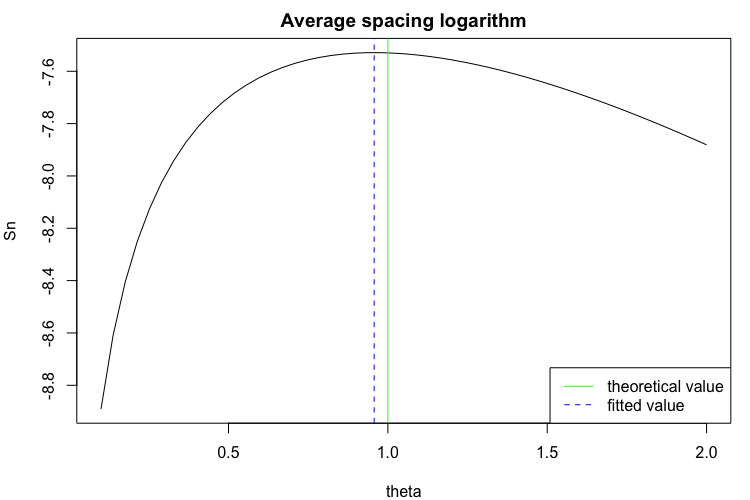
\includegraphics[width=1\textwidth]{img/exp-ASL}



\end{frame}

\begin{frame}{Example 1 -- std. exponential distribution -- gof. plots}


\centering

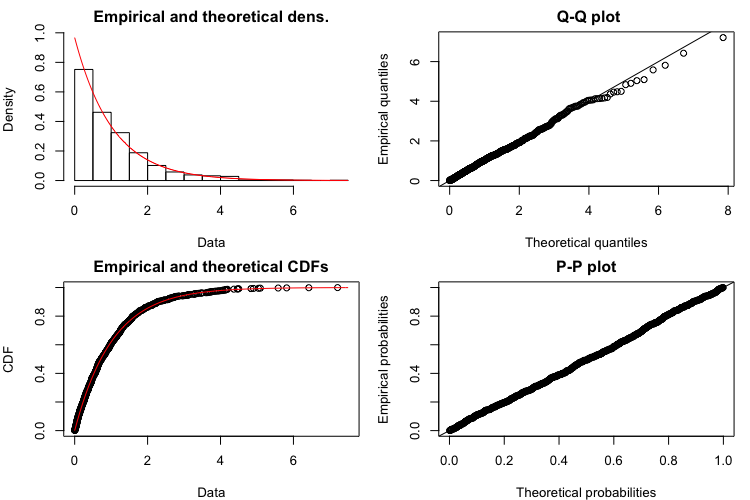
\includegraphics[width=\textwidth]{img/exp-plotdist}


\end{frame}

\begin{frame}{Example 2 -- Burr distribution -- gof. plots}
Simulated dataset from $\mathcal Burr(2,2,2)$ and $n=10000$.

\centering
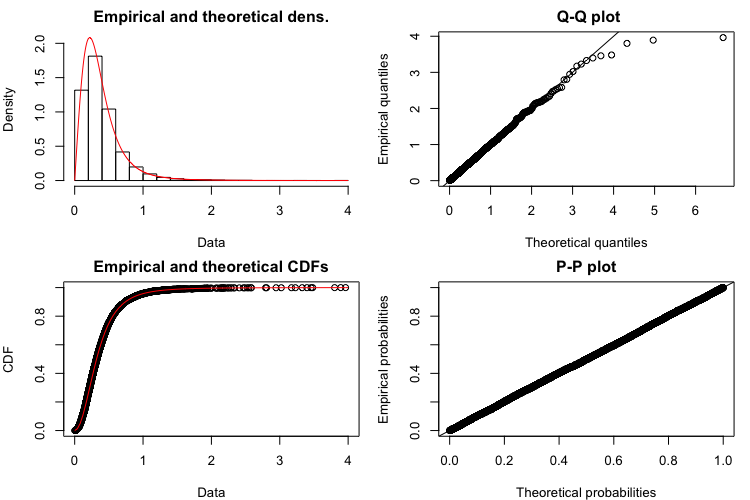
\includegraphics[width=\textwidth]{img/burr-plotdist}


\end{frame}

\begin{frame}{Example 2 -- Burr distribution -- bootstrap}

\centering
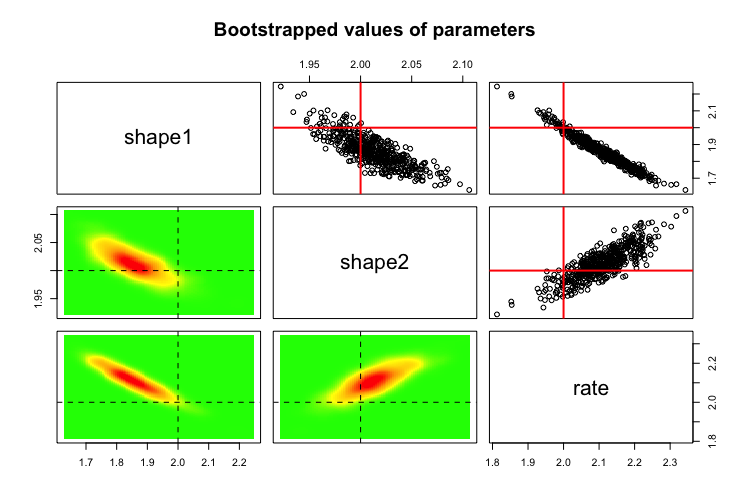
\includegraphics[width=1.05\textwidth]{img/burr-bootdist}

\end{frame}


\begin{frame}{Example 3 -- real dataset}
Consider Normalized Hurricane Damages in the United States: 1900-2005 used in Pielke et al. (2008).

\centering
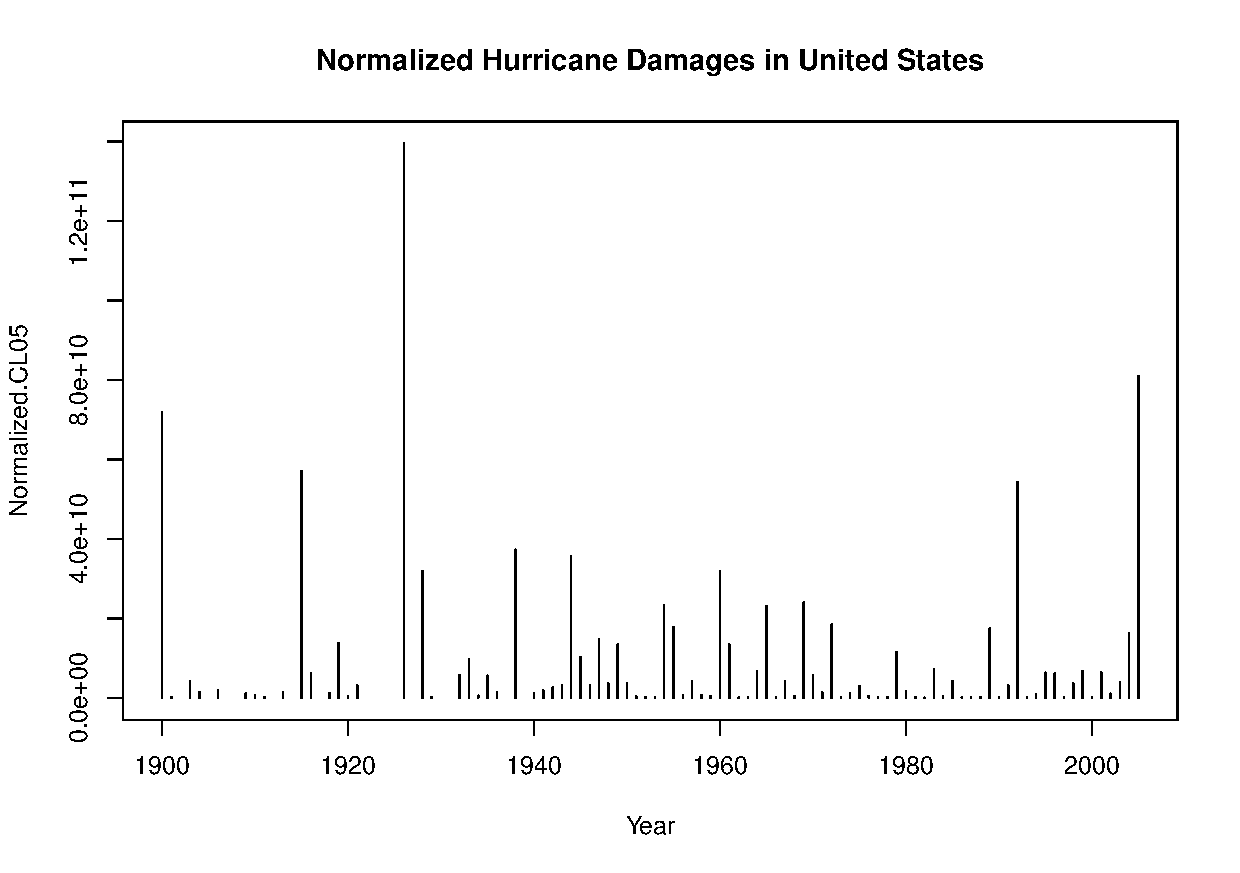
\includegraphics[width=\textwidth]{img/Ushustorm}

\end{frame}



\begin{frame}{Example 3 -- real dataset -- graphics}

\begin{tabular}{cc}
\hspace{-.5cm}
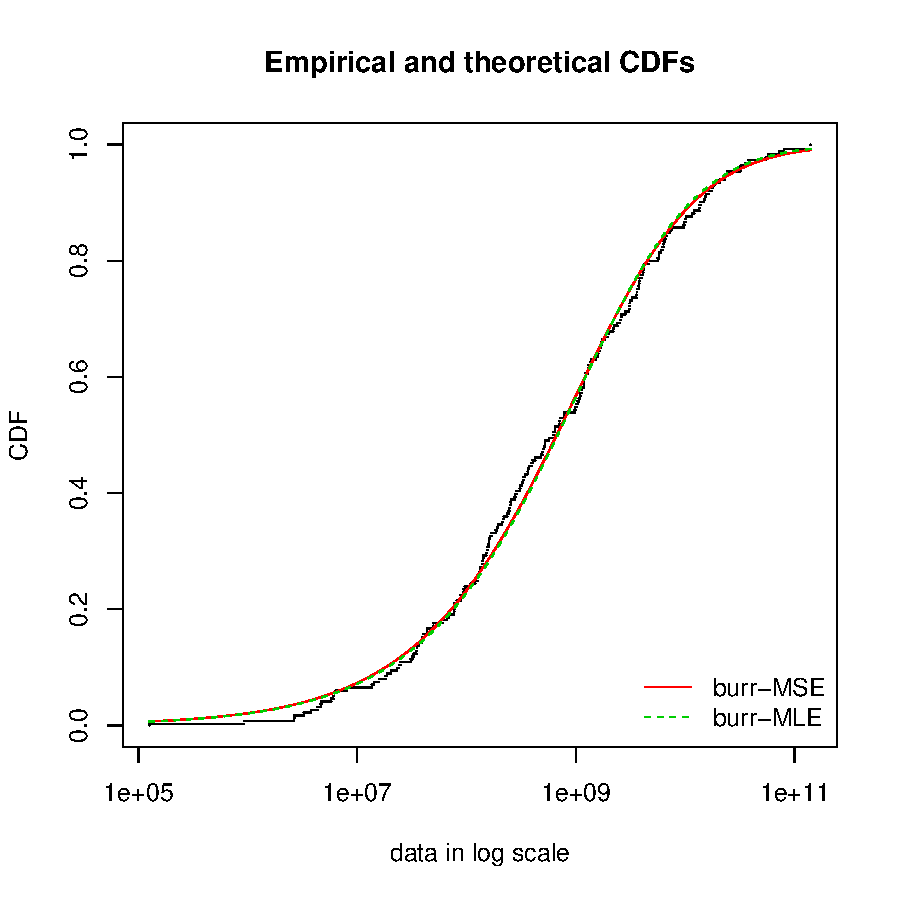
\includegraphics[width=.55\textwidth]{img/Ushustorm-cdfcomp}&
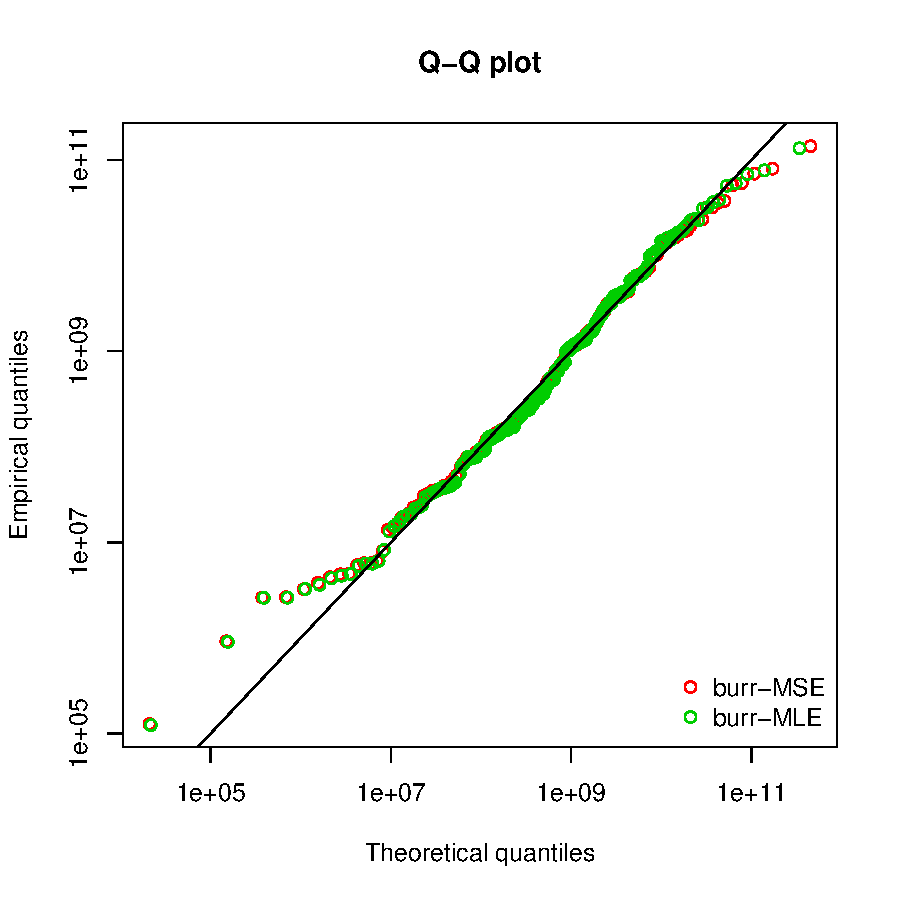
\includegraphics[width=.55\textwidth]{img/Ushustorm-qqcomp}
\end{tabular}

\end{frame}

\begin{frame}{Example 3 -- real dataset -- gof. statistics for burr distribution}
\centering
Coefficients values\\
\begin{tabular}{rrr}
  \hline
 & MSE & MLE \\ 
  \hline
shape1 & 2.2075 & 2.4563 \\ 
  shape2 & 0.5611 & 0.5604 \\ 
  rate & 2.5318e-10 & 1.9825e-10 \\ 
   \hline
\end{tabular}
\bigskip

Goodness-of-fit statistics\\
\begin{tabular}{ccc}
                             & MSE & MLE \\
\hline                             
Kolmogorov-Smirnov statistic &0.04421733 &0.04867166 \\
\hline                             
Cramer-von Mises statistic   &0.06798511 &0.08520099 \\
\hline                             
Anderson-Darling statistic   &0.43766768 &0.51206510 \\
\hline                             
\end{tabular}
\bigskip

Goodness-of-fit criteria\\
\begin{tabular}{ccc}
                             & MSE & MLE \\
\hline                             
Akaike's Information Criterion   &9301.882   &9301.723 \\
\hline                             
Bayesian Information Criterion   &9311.880   &9311.721 \\
\hline                             
\end{tabular}
\end{frame}



%________________________________________________________________
\section{Conclusion and perspectives}

\begin{frame}{Conclusion and perspectives}

We implements (very quickly) in \pkg{fitdistrplus}
\begin{itemize}
\item a new statistical procedure Maximum Spacing Estimation.
\item[]
\item as well as the generalized Maximum Spacing Estimation considering $\phi$ divergence function.
\item[]
\item automatically all generic functions (\code{plot}, \code{summary}, \code{coef},\dots) are available.
\end{itemize}

\end{frame}


\begin{frame}{References}
    
  
  \begin{thebibliography}{1}
 \begin{footnotesize}
 
 
  
  
  \beamertemplatearticlebibitems
	
\bibitem{ranneby}
Cheng, R.C.H., Amin, N.A.K. (1983),
  \newblock Estimating parameters in continuous univariate distributions with a shifted origin,
  \newblock {\em Journal of the Royal Statistical Society Ser. B}, 45, 394-403.
	
  
\bibitem{ranneby}
Ranneby B (1984),
  \newblock The Maximum Spacing Method. An Estimation Method Related to the Maximum Likelihood Method,
  \newblock {\em Scandinavian Journal of Statistics}, 11(2),  93-112 

\bibitem{rannebyekstrom}
Ranneby B \& Ekstrom M (1997), 
\newblock Maximum spacing estimates based on different metrics, 
  \newblock {\em Umea universitet},  research paper.	

  

  
\bibitem{ekstrom}
Ekstrom M (2015), 
\newblock On the consistency of the maximum spacing method, 
  \newblock {\em Journal of Statistical Planning and Inference}, 70, 209-224.	
  
  
  
\setbeamertemplate{bibliography item}[online]



\bibitem{fitdistrplus}
Delignette-Muller ML \& Dutang C (2019), 
\newblock   fitdistrplus: An R Package for Fitting Distributions,
\newblock \url{https://CRAN.R-project.org/package=fitdistrplus}

 \bibitem{MPS}
 Teimouri M. (2018), 
\newblock  MPS: Estimating Through the Maximum Product Spacing Approach,
\newblock \url{https://CRAN.R-project.org/package=MPS}


 \bibitem{BMT}
Torres-Jimenez C.J. (2017), 
\newblock  BMT: The BMT Distribution,
\newblock \url{https://CRAN.R-project.org/package=BMT}


  

     
  \end{footnotesize}
\end{thebibliography}
  
   
\end{frame}

%
%\appendix
%\backupbegin
%
%
%%%%%%%%%%%%%%%%%%%%%%%%%%%%%%%%%%%%%%%
%\section*{Annexes}
%%%%%%%%%%%%%%%%%%%%%%%%%%%%%%%%%%%%%%%
%\subsection*{Annexes}
%
%
%\begin{frame}{Model diagnostics -- residuals}
%
%
%
%\end{frame}
%
%
%
%
%
%\backupend



%---------------------------- End of presentation body
\end{document}


